\documentclass[12pt]{scrartcl}
\usepackage[hagavi]{azzam}
\usetikzlibrary{calc,intersections,angles,quotes,through}

% titik hitam kecil di setiap koordinat yang disebut
\newcommand{\titik}[1]{\foreach \p in {#1} \filldraw (\p) circle (1.4pt);}

\title{Geometri Pelatda OSN SMA 2026}
\author{Azzam Labib Hakim}
\date{10 September 2026}

\begin{document}
\maketitle

Tiga kelompok teknik di bawah ini menutupi sebagian besar soal geometri OSN. Angle chasing dipakai untuk mengejar kesiklisan dan kesejajaran, homoteti dipakai saat ada dua bangun sebangun yang posisinya searah, dan length chasing dipakai kalau yang diminta soal adalah hubungan panjang. Yang perlu kalian bangun bukan hafalan lemma, melainkan refleks memilih salah satu dari tiga jalur ini dalam lima belas menit pertama.

Setiap grup ditutup dengan latihan soal. Kerjakan gambarnya besar dan rapi sebelum menulis apa pun.

\renewcommand*\contentsname{Daftar Isi}
\tableofcontents
\newpage

\section{Angle Chasing}

\subsection{Phantom Point}

\begin{definition*}[Phantom point]
Misalkan kita diminta membuktikan bahwa suatu titik $X$ punya sifat $\mathcal{P}$, dan sifat $\mathcal{P}$ itu sendiri sudah cukup untuk menentukan sebuah titik secara tunggal. Alih alih menyerang $X$ langsung, definisikan titik baru $X'$ yang memenuhi $\mathcal{P}$, lalu buktikan $X' = X$. Titik $X'$ inilah yang disebut \emph{phantom point} atau titik bayangan.
\end{definition*}

Kunci teknik ini ada pada ketunggalan. Dua garis yang tidak sejajar berpotongan tepat di satu titik, sebuah garis memotong lingkaran paling banyak di dua titik, dan busur punya tepat satu titik tengah. Begitu $X'$ dan $X$ terbukti memenuhi kondisi ketunggalan yang sama, keduanya wajib berimpit.

\begin{lemma*}[Pencerminan titik tinggi terhadap sisi]
Diberikan $\triangle ABC$ dengan titik tinggi $H$. Pencerminan $H$ terhadap garis $BC$ terletak pada lingkaran luar $\triangle ABC$.
\end{lemma*}

\begin{figure}[H]
\centering
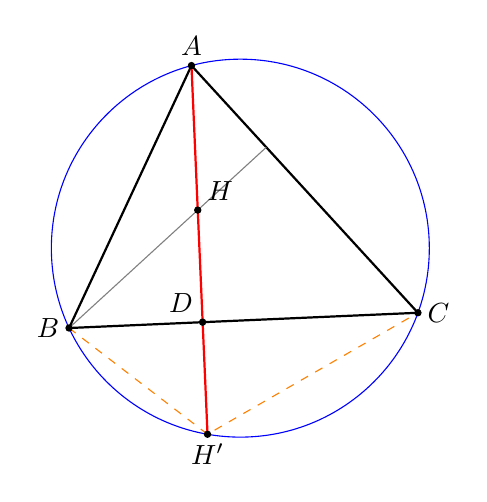
\begin{tikzpicture}[scale=0.8]
  \coordinate (O)  at (0,0);
  \coordinate (A)  at (-0.776,2.898);
  \coordinate (B)  at (-2.719,-1.268);
  \coordinate (C)  at (2.819,-1.026);
  \coordinate (H)  at (-0.676,0.604);
  \coordinate (D)  at (-0.599,-1.175);
  \coordinate (Hb) at (-0.521,-2.954);
  \coordinate (E)  at (0.412,1.601);

  \draw[blue] (O) circle (3);
  \draw[thick] (A) -- (B) -- (C) -- cycle;
  \draw[red,thick] (A) -- (Hb);
  \draw[gray] (B) -- (E);
  \draw[orange,dashed] (B) -- (Hb) -- (C);

  \titik{A,B,C,H,D,Hb}
  \node[above]       at (A)  {$A$};
  \node[left]        at (B)  {$B$};
  \node[right]       at (C)  {$C$};
  \node[above right] at (H)  {$H$};
  \node[above left]  at (D)  {$D$};
  \node[below]       at (Hb) {$H'$};
\end{tikzpicture}
\caption{$H'$ adalah pencerminan $H$ terhadap $BC$, dan ia mendarat di lingkaran luar.}
\end{figure}

\begin{proof}
Misalkan $D$ kaki garis tinggi dari $A$, dan definisikan $H'$ sebagai pencerminan $H$ terhadap $BC$. Kita akan menunjukkan $ABH'C$ siklis, sehingga $H'$ berimpit dengan perpotongan kedua garis $AD$ dengan lingkaran luar.

Dari $\angle HBC = 90^\circ - \angle C$ dan $\angle HCB = 90^\circ - \angle B$ kita peroleh
\[
\angle BHC = 180^\circ - \angle HBC - \angle HCB = \angle B + \angle C = 180^\circ - \angle A.
\]
Pencerminan mempertahankan besar sudut, jadi $\angle BH'C = \angle BHC = 180^\circ - \angle A$. Akibatnya $\angle BAC + \angle BH'C = 180^\circ$, yang berarti $ABH'C$ siklis.

Sekarang $H'$ terletak pada garis $AD$ (karena $H$ dan $H'$ simetris terhadap $BC$ dan $AD \perp BC$) sekaligus pada lingkaran luar. Garis $AD$ memotong lingkaran luar di $A$ dan satu titik lain saja, dan $H' \ne A$. Jadi $H'$ tepat titik potong kedua tersebut.
\end{proof}

Perhatikan alur berpikirnya. Kita tidak pernah menghitung apa pun tentang titik potong kedua garis $AD$ dengan lingkaran luar. Kita membuat titik tandingannya, membuktikan ia siklis, lalu memakai ketunggalan untuk menutup argumen. Pola yang sama muncul lagi di \S\ref{sec:talibusur} untuk membuktikan kolinearitas $T$, $K$, $M$.

\subsection{Sudut Isogonal: $\angle BAH = \angle CAO$}

\begin{theorem*}
Pada $\triangle ABC$ dengan titik tinggi $H$ dan titik pusat lingkaran luar $O$, garis $AH$ dan garis $AO$ simetris terhadap garis bagi $\angle A$. Ekuivalen, $\angle BAH = \angle CAO$.
\end{theorem*}

\begin{figure}[H]
\centering
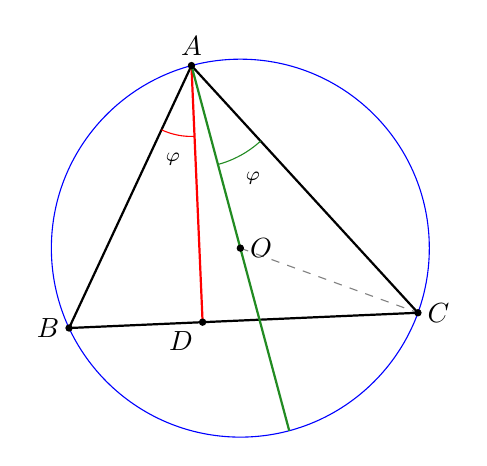
\begin{tikzpicture}[scale=0.8]
  \coordinate (O)  at (0,0);
  \coordinate (A)  at (-0.776,2.898);
  \coordinate (B)  at (-2.719,-1.268);
  \coordinate (C)  at (2.819,-1.026);
  \coordinate (D)  at (-0.599,-1.175);
  \coordinate (Ab) at (0.776,-2.898);

  \draw[blue] (O) circle (3);
  \draw[thick] (A) -- (B) -- (C) -- cycle;
  \draw[red,thick] (A) -- (D);
  \draw[ForestGreen,thick] (A) -- (Ab);
  \draw[gray,dashed] (O) -- (C);

  \pic[draw=red,angle radius=9mm,"\scriptsize$\varphi$",angle eccentricity=1.35]
      {angle=B--A--D};
  \pic[draw=ForestGreen,angle radius=13mm,"\scriptsize$\varphi$",angle eccentricity=1.25]
      {angle=Ab--A--C};

  \titik{A,B,C,D,O}
  \node[above]       at (A) {$A$};
  \node[left]        at (B) {$B$};
  \node[right]       at (C) {$C$};
  \node[below left]  at (D) {$D$};
  \node[right]       at (O) {$O$};
\end{tikzpicture}
\caption{Garis tinggi $AD$ dan jari jari $AO$ membentuk sudut yang sama terhadap $AB$ dan $AC$.}
\end{figure}

\begin{proof}
Misalkan $D$ kaki garis tinggi dari $A$. Pada $\triangle ABD$ yang siku siku di $D$,
\[
\angle BAD = 90^\circ - \angle B.
\]
Di sisi lain, sudut pusat $\angle AOC$ menghadap busur $AC$ yang sama dengan sudut keliling $\angle ABC$, jadi $\angle AOC = 2\angle B$. Karena $OA = OC = R$, segitiga $AOC$ sama kaki dan
\[
\angle OAC = \frac{180^\circ - 2\angle B}{2} = 90^\circ - \angle B.
\]
Kedua sudut bernilai sama, jadi $\angle BAH = \angle BAD = \angle OAC = \angle CAO$.
\end{proof}

Konsekuensinya sering lebih berguna daripada pernyataannya. Kalau $AI$ adalah garis bagi $\angle A$, maka $AI$ juga garis bagi $\angle HAO$. Dari sini lahir fakta bahwa $I$ terletak di antara $H$ dan $O$ dalam pengertian sudut, dan bahwa $AH = AO$ tepat ketika $\angle A = 60^\circ$.

\subsection{Pencerminan Titik Tinggi terhadap Titik Tengah Sisi}

\begin{theorem*}
Misalkan $M$ titik tengah $BC$ dan $A'$ titik antipoda $A$ pada lingkaran luar $\triangle ABC$. Maka $M$ adalah titik tengah $HA'$, dan $BHCA'$ jajar genjang.
\end{theorem*}

\begin{figure}[H]
\centering
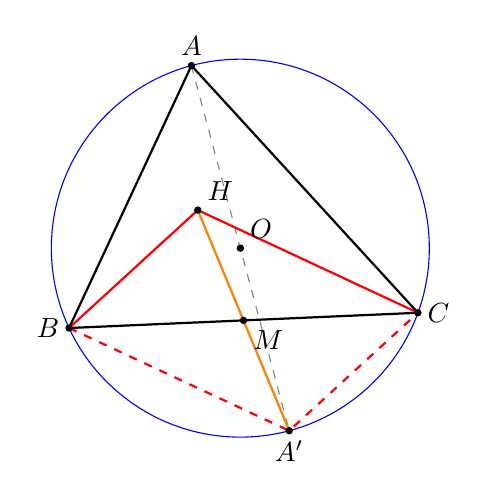
\begin{tikzpicture}[scale=0.8]
  \coordinate (O)  at (0,0);
  \coordinate (A)  at (-0.776,2.898);
  \coordinate (B)  at (-2.719,-1.268);
  \coordinate (C)  at (2.819,-1.026);
  \coordinate (H)  at (-0.676,0.604);
  \coordinate (M)  at (0.050,-1.147);
  \coordinate (Ab) at (0.776,-2.898);

  \draw[blue] (O) circle (3);
  \draw[thick] (A) -- (B) -- (C) -- cycle;
  \draw[gray,dashed] (A) -- (Ab);
  \draw[red,thick] (B) -- (H) -- (C);
  \draw[red,thick,dashed] (B) -- (Ab) -- (C);
  \draw[orange,thick] (H) -- (Ab);

  \titik{A,B,C,H,M,O,Ab}
  \node[above]       at (A)  {$A$};
  \node[left]        at (B)  {$B$};
  \node[right]       at (C)  {$C$};
  \node[above right] at (H)  {$H$};
  \node[below right] at (M)  {$M$};
  \node[above right] at (O)  {$O$};
  \node[below]       at (Ab) {$A'$};
\end{tikzpicture}
\caption{$BHCA'$ jajar genjang, sehingga $M$ sekaligus titik tengah $BC$ dan titik tengah $HA'$.}
\end{figure}

\begin{proof}
Karena $AA'$ diameter, $\angle ACA' = 90^\circ$, jadi $A'C \perp AC$. Garis tinggi dari $B$ juga tegak lurus $AC$, sehingga $BH \parallel A'C$. Dengan cara yang sama $\angle ABA' = 90^\circ$ memberi $A'B \perp AB$, sedangkan $CH \perp AB$, jadi $CH \parallel A'B$.

Kedua pasang sisi berhadapan pada segiempat $BHCA'$ sejajar, jadi ia jajar genjang. Diagonalnya, yaitu $BC$ dan $HA'$, saling membagi dua sama panjang di $M$.
\end{proof}

\subsection{Jarak Titik Sudut ke Titik Tinggi: $AH = 2 \cdot OM$}

\begin{theorem*}
Pada $\triangle ABC$ dengan titik tinggi $H$, titik pusat lingkaran luar $O$, dan $M$ titik tengah $BC$, berlaku $AH = 2 \cdot OM$ dan $AH \parallel OM$.
\end{theorem*}

\begin{figure}[H]
\centering
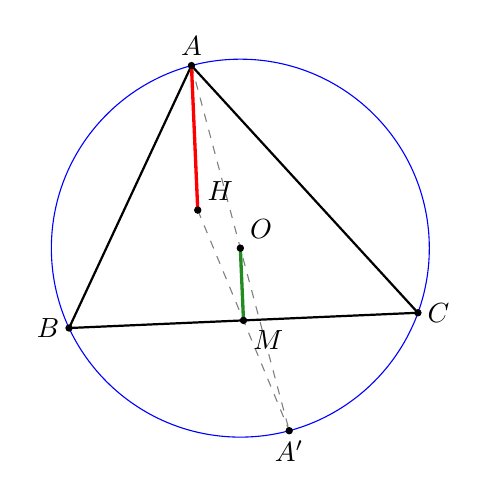
\begin{tikzpicture}[scale=0.8]
  \coordinate (O)  at (0,0);
  \coordinate (A)  at (-0.776,2.898);
  \coordinate (B)  at (-2.719,-1.268);
  \coordinate (C)  at (2.819,-1.026);
  \coordinate (H)  at (-0.676,0.604);
  \coordinate (M)  at (0.050,-1.147);
  \coordinate (Ab) at (0.776,-2.898);

  \draw[blue] (O) circle (3);
  \draw[thick] (A) -- (B) -- (C) -- cycle;
  \draw[gray,dashed] (A) -- (Ab);
  \draw[gray,dashed] (H) -- (Ab);
  \draw[red,very thick] (A) -- (H);
  \draw[ForestGreen,very thick] (O) -- (M);

  \titik{A,B,C,H,M,O,Ab}
  \node[above]       at (A)  {$A$};
  \node[left]        at (B)  {$B$};
  \node[right]       at (C)  {$C$};
  \node[above right] at (H)  {$H$};
  \node[below right] at (M)  {$M$};
  \node[above right] at (O)  {$O$};
  \node[below]       at (Ab) {$A'$};
\end{tikzpicture}
\caption{$OM$ adalah garis tengah $\triangle AHA'$, jadi panjangnya separuh $AH$.}
\end{figure}

\begin{proof}
Pakai hasil sebelumnya: $M$ adalah titik tengah $HA'$, dengan $A'$ antipoda $A$. Pada $\triangle AHA'$, titik $O$ adalah titik tengah $AA'$ dan $M$ titik tengah $HA'$. Jadi $OM$ merupakan garis tengah segitiga tersebut, yang berarti $OM \parallel AH$ dan $AH = 2 \cdot OM$.
\end{proof}

Rumus ini yang membuat $AH = 2R\cos A$, karena $OM = R \cos A$ dari segitiga siku siku $OMB$. Kalau dalam suatu soal muncul jarak titik sudut ke titik tinggi, hampir selalu bentuk $2R \cos A$ inilah yang dipakai.

\subsection{Incenter Excenter Lemma}
\label{sec:incenter-excenter}

\begin{theorem*}[Lemma kutub selatan]
Misalkan $I$ titik pusat lingkaran dalam $\triangle ABC$ dan $I_A$ titik pusat lingkaran singgung luar yang menyinggung sisi $BC$. Jika garis bagi $\angle A$ memotong lingkaran luar lagi di $M$, maka
\[
MB = MI = MC = MI_A.
\]
Dengan kata lain, $M$ adalah pusat lingkaran yang melalui $B$, $I$, $C$, dan $I_A$.
\end{theorem*}

\begin{figure}[H]
\centering
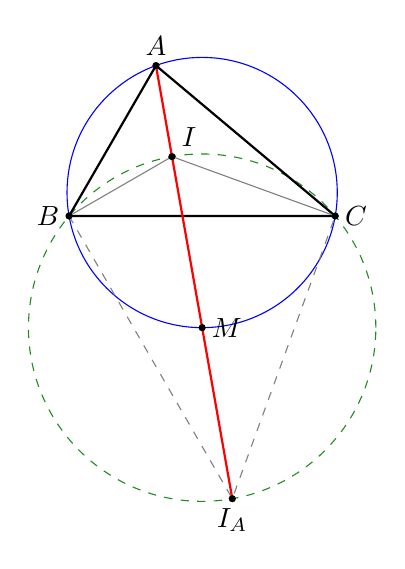
\begin{tikzpicture}[scale=0.78]
  \coordinate (O)  at (0,0);
  \coordinate (A)  at (-0.752,2.067);
  \coordinate (B)  at (-2.167,-0.382);
  \coordinate (C)  at (2.167,-0.382);
  \coordinate (I)  at (-0.491,0.585);
  \coordinate (M)  at (0,-2.2);
  \coordinate (Ia) at (0.491,-4.985);

  \draw[blue] (O) circle (2.2);
  \draw[ForestGreen,dashed] (M) circle (2.828);
  \draw[thick] (A) -- (B) -- (C) -- cycle;
  \draw[red,thick] (A) -- (Ia);
  \draw[gray] (B) -- (I) -- (C);
  \draw[gray,dashed] (B) -- (Ia) -- (C);

  \titik{A,B,C,I,M,Ia}
  \node[above]       at (A)  {$A$};
  \node[left]        at (B)  {$B$};
  \node[right]       at (C)  {$C$};
  \node[above right] at (I)  {$I$};
  \node[right]       at (M)  {$M$};
  \node[below]       at (Ia) {$I_A$};
\end{tikzpicture}
\caption{Titik tengah busur $BC$ menjadi pusat satu lingkaran yang memuat $B$, $I$, $C$, dan $I_A$.}
\end{figure}

\begin{proof}
Tulis $\angle A = 2\alpha$, $\angle B = 2\beta$, $\angle C = 2\gamma$. Karena $AM$ garis bagi $\angle A$, titik $M$ adalah titik tengah busur $BC$ yang tidak memuat $A$, sehingga $\angle MBC = \angle MAC = \alpha$. Maka
\[
\angle MBI = \angle MBC + \angle CBI = \alpha + \beta.
\]
Di sisi lain, $\angle MIB$ adalah sudut luar $\triangle ABI$ di titik $I$, jadi
\[
\angle MIB = \angle IAB + \angle IBA = \alpha + \beta.
\]
Kedua sudut sama, jadi $\triangle MBI$ sama kaki dengan $MB = MI$. Argumen simetris memberi $MC = MI$.

Untuk $I_A$, ingat bahwa $BI$ adalah garis bagi dalam $\angle B$ sedangkan $BI_A$ garis bagi luarnya, sehingga $\angle IBI_A = 90^\circ$. Titik $I$, $M$, $I_A$ segaris karena ketiganya ada pada garis bagi $\angle A$. Jadi $\triangle IBI_A$ siku siku di $B$ dengan hipotenusa $II_A$, dan $M$ pada hipotenusa itu memenuhi $MB = MI$. Titik tengah hipotenusa adalah satu satunya titik pada hipotenusa yang berjarak sama ke $B$ dan ke $I$, jadi $M$ titik tengah $II_A$ dan $MI_A = MI = MB$.
\end{proof}

\subsection{Latihan Soal Angle Chasing}

\begin{enumerate}
  \item (OSP 2017) Diberikan segitiga $ABC$ yang ketiga garis tingginya berpotongan di titik $H$. Tentukan semua titik $X$ pada sisi $BC$ sehingga pencerminan $H$ terhadap titik $X$ terletak pada lingkaran luar segitiga $ABC$.

  \item Segitiga $ABC$ memiliki titik tinggi $H$ dan titik pusat lingkaran dalam $I$. Buktikan bahwa $A$, $B$, $H$, $I$ konsiklis jika dan hanya jika $\angle ACB = 60^\circ$.

  \item Misalkan $C$ adalah titik pada setengah lingkaran berdiameter $AB$, terletak pada busurnya dan bukan pada diameternya. Misalkan $D$ titik tengah busur $AC$. Notasikan $E$ sebagai proyeksi $D$ pada garis $BC$, dan $F$ perpotongan $AE$ dengan setengah lingkaran tersebut. Buktikan bahwa $BF$ membagi $DE$ sama panjang.

  \item (OSN 2002) Diberikan segitiga $ABC$ dengan $AC > BC$. Pada lingkaran luar segitiga $ABC$ terletak titik $D$ yang merupakan titik tengah busur $AB$ yang memuat titik $C$. Misalkan $E$ titik pada $AC$ sehingga $DE$ tegak lurus $AC$. Buktikan bahwa $AE = EC + CB$.

  \item (OSN 2007) Titik $A$, $B$, $C$, $D$ terletak pada lingkaran $S$ sedemikian sehingga $AB$ merupakan diameter $S$, tetapi $CD$ bukan diameter $S$. Diketahui pula $C$ dan $D$ berada pada sisi berbeda terhadap $AB$. Garis singgung terhadap $S$ di $C$ dan di $D$ berpotongan di titik $P$. Titik $Q$ dan $R$ berturut turut adalah perpotongan garis $AC$ dengan $BD$ dan perpotongan garis $AD$ dengan $BC$. Buktikan bahwa $P$, $Q$, $R$ segaris, lalu buktikan bahwa $QR \perp AB$.

  \item (OSN 2009) Diberikan segitiga lancip $ABC$. Lingkaran dalamnya menyinggung $BC$, $CA$, $AB$ berturut turut di $D$, $E$, $F$. Garis bagi $\angle A$ memotong $DE$ dan $DF$ berturut turut di $K$ dan $L$. Misalkan $AA_1$ garis tinggi dan $M$ titik tengah $BC$.
  \begin{enumerate}
    \item[(a)] Buktikan bahwa $BK$ dan $CL$ tegak lurus garis bagi $\angle BAC$.
    \item[(b)] Tunjukkan bahwa $A_1KML$ adalah segiempat talibusur.
  \end{enumerate}

  \item (OSN 2015) Diberikan segitiga lancip $ABC$ dengan titik pusat lingkaran luar $O$. Garis $AO$ memotong lingkaran luar segitiga $ABC$ lagi di titik $D$. Misalkan $P$ titik pada sisi $BC$. Garis melalui $P$ yang tegak lurus $AP$ memotong garis $DB$ dan $DC$ berturut turut di $E$ dan $F$. Garis melalui $D$ yang tegak lurus $BC$ memotong $EF$ di $Q$. Buktikan bahwa $EQ = FQ$ jika dan hanya jika $BP = CP$.

  \item (IMO 2006) Diberikan segitiga $ABC$ dengan titik pusat lingkaran dalam $I$. Titik $P$ di dalam segitiga memenuhi
  \[
  \angle PBA + \angle PCA = \angle PBC + \angle PCB.
  \]
  Buktikan bahwa $AP \ge AI$, dan kesamaan terjadi tepat ketika $P = I$.

  \item (IMO SL 2010) Let $\triangle ABC$ be an acute triangle with $D$, $E$, $F$ the feet of the altitudes lying on $\overline{BC}$, $\overline{CA}$, and $\overline{AB}$ respectively. One of the intersection points of the line $\overline{EF}$ and the circumcircle is $P$. The lines $\overline{BP}$ and $\overline{DF}$ meet at point $Q$. Prove that $|AP| = |AQ|$.

  \item (Korea 2022) Let $ABC$ be an acute triangle with circumcenter $O$, and let $D$, $E$, and $F$ be the feet of altitudes from $A$, $B$, and $C$ to sides $BC$, $CA$, and $AB$, respectively. Denote by $P$ the intersection of the tangents to the circumcircle of $ABC$ at $B$ and $C$. The line through $P$ perpendicular to $EF$ meets $AD$ at $Q$, and let $R$ be the foot of the perpendicular from $A$ to $EF$. Prove that $DR$ and $OQ$ are parallel.
\end{enumerate}

\newpage
\section{Homoteti}

Homoteti, atau dilatasi kalau memakai istilah kurikulum sekolah, adalah transformasi yang mengubah ukuran sebuah bangun tanpa mengubah bentuknya. Ia ditentukan oleh dua data saja:
\begin{enumerate}
  \item \textbf{Titik pusat} $O$, satu satunya titik yang tidak berpindah.
  \item \textbf{Faktor skala} $k$, bilangan real tak nol yang menentukan seberapa besar perubahan ukuran sekaligus arah pemetaannya.
\end{enumerate}

Homoteti dengan pusat $O$ dan faktor $k$ memetakan setiap titik $P$ ke $P'$ dengan
\[
\vec{OP'} = k \cdot \vec{OP}.
\]

Tanda $k$ menentukan letak bayangan. Untuk $k > 0$ bayangan berada pada sinar yang sama dengan aslinya dari $O$, membesar kalau $k > 1$ dan mengecil kalau $0 < k < 1$. Untuk $k < 0$ bayangan menyeberang ke sisi lain $O$, jadi bangunnya ikut terbalik.

\begin{figure}[H]
\centering
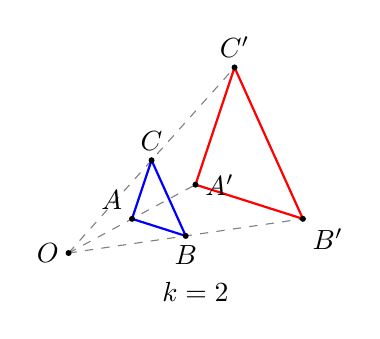
\begin{tikzpicture}[scale=0.62]
  \coordinate (O)  at (0,0);
  \coordinate (A)  at (1.3,0.7);
  \coordinate (B)  at (2.4,0.35);
  \coordinate (C)  at (1.7,1.9);
  \coordinate (Ab) at (2.6,1.4);
  \coordinate (Bb) at (4.8,0.7);
  \coordinate (Cb) at (3.4,3.8);

  \draw[gray,dashed] (O) -- (Ab);
  \draw[gray,dashed] (O) -- (Bb);
  \draw[gray,dashed] (O) -- (Cb);
  \draw[thick,blue] (A) -- (B) -- (C) -- cycle;
  \draw[thick,red] (Ab) -- (Bb) -- (Cb) -- cycle;

  \titik{O,A,B,C,Ab,Bb,Cb}
  \node[left]        at (O)  {$O$};
  \node[above left]  at (A)  {$A$};
  \node[below]       at (B)  {$B$};
  \node[above]       at (C)  {$C$};
  \node[right]       at (Ab) {$A'$};
  \node[below right] at (Bb) {$B'$};
  \node[above]       at (Cb) {$C'$};
  \node at (2.6,-0.8) {$k = 2$};
\end{tikzpicture}
\hspace{1.2cm}
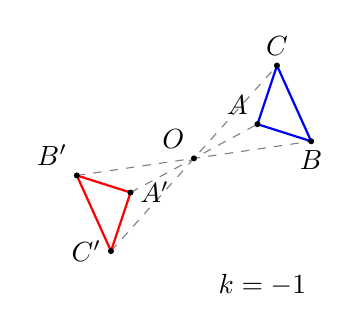
\begin{tikzpicture}[scale=0.62]
  \coordinate (O)  at (0,0);
  \coordinate (A)  at (1.3,0.7);
  \coordinate (B)  at (2.4,0.35);
  \coordinate (C)  at (1.7,1.9);
  \coordinate (Ab) at (-1.3,-0.7);
  \coordinate (Bb) at (-2.4,-0.35);
  \coordinate (Cb) at (-1.7,-1.9);

  \draw[gray,dashed] (Ab) -- (A);
  \draw[gray,dashed] (Bb) -- (B);
  \draw[gray,dashed] (Cb) -- (C);
  \draw[thick,blue] (A) -- (B) -- (C) -- cycle;
  \draw[thick,red] (Ab) -- (Bb) -- (Cb) -- cycle;

  \titik{O,A,B,C,Ab,Bb,Cb}
  \node[above left]  at (O)  {$O$};
  \node[above left]  at (A)  {$A$};
  \node[below]       at (B)  {$B$};
  \node[above]       at (C)  {$C$};
  \node[right]       at (Ab) {$A'$};
  \node[above left]  at (Bb) {$B'$};
  \node[left]        at (Cb) {$C'$};
  \node at (1.4,-2.6) {$k = -1$};
\end{tikzpicture}
\caption{Homoteti berpusat $O$ dengan faktor positif dan faktor negatif.}
\end{figure}

Yang membuat homoteti berguna di olimpiade adalah kebalikannya. Kalau ada dua lingkaran yang bersinggungan, titik singgungnya otomatis menjadi pusat homoteti yang memetakan satu lingkaran ke lingkaran lainnya. Begitu pusat homoteti ditemukan, semua garis penghubung titik asal dengan bayangannya melalui titik itu, dan setiap garis singgung terpetakan ke garis singgung yang sejajar. Dua kesimpulan gratis inilah yang biasanya menyelesaikan soal.

\subsection{Lingkaran yang Menyinggung Tali Busur}
\label{sec:talibusur}

\begin{theorem*}[Lemma Archimedes]
Diberikan lingkaran $\Omega$ dengan tali busur $AB$. Misalkan $\omega$ lingkaran yang menyinggung $AB$ di $K$ dan menyinggung $\Omega$ dari dalam di $T$. Misalkan $M$ titik tengah busur $AB$ yang tidak memuat $T$. Maka $T$, $K$, $M$ segaris, dan
\[
MK \cdot MT = MB^2 = MA^2.
\]
\end{theorem*}

\begin{figure}[H]
\centering
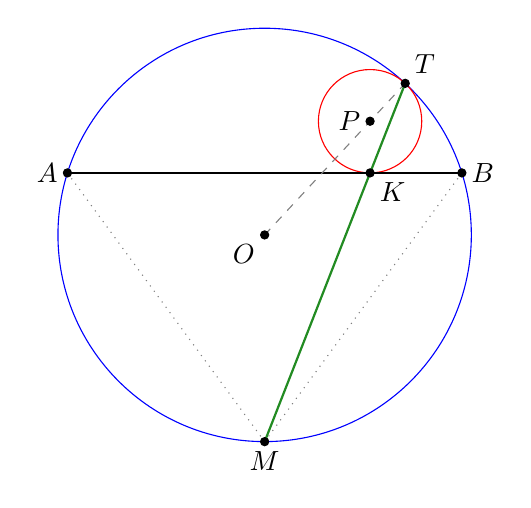
\begin{tikzpicture}[scale=1.05]
  \coordinate (O) at (0,0);
  \coordinate (P) at (1.275,1.375);
  \coordinate (A) at (-2.385,0.75);
  \coordinate (B) at (2.385,0.75);
  \coordinate (K) at (1.275,0.75);
  \coordinate (T) at (1.700,1.833);
  \coordinate (M) at (0,-2.5);

  \draw[blue] (O) circle (2.5);
  \draw[red] (P) circle (0.625);
  \draw[thick] (A) -- (B);
  \draw[ForestGreen,thick] (M) -- (T);
  \draw[gray,dotted] (M) -- (A);
  \draw[gray,dotted] (M) -- (B);
  \draw[gray,dashed] (O) -- (T);

  \titik{A,B,K,T,M,O,P}
  \node[left]        at (A) {$A$};
  \node[right]       at (B) {$B$};
  \node[below right] at (K) {$K$};
  \node[above right] at (T) {$T$};
  \node[below]       at (M) {$M$};
  \node[below left]  at (O) {$O$};
  \node[left]        at (P) {$P$};
\end{tikzpicture}
\caption{Homoteti berpusat $T$ memetakan $\omega$ ke $\Omega$ dan membawa $K$ ke $M$.}
\end{figure}

\begin{proof}
Kedua lingkaran bersinggungan dalam di $T$, jadi pusat $\omega$, pusat $\Omega$, dan $T$ segaris. Akibatnya ada homoteti $h$ berpusat $T$ dengan faktor positif yang memetakan $\omega$ ke $\Omega$.

Pakai phantom point. Definisikan $M' = h(K)$, yaitu titik potong kedua garis $TK$ dengan $\Omega$. Homoteti memetakan garis singgung $\omega$ di $K$ ke garis singgung $\Omega$ di $M'$, dan kedua garis itu sejajar. Garis singgung $\omega$ di $K$ tidak lain adalah $AB$, jadi garis singgung $\Omega$ di $M'$ sejajar $AB$. Hanya ada dua titik pada $\Omega$ dengan garis singgung sejajar $AB$, yaitu kedua titik tengah busur $AB$. Karena $M'$ berada di sisi $AB$ yang berseberangan dengan $T$, titik $M'$ adalah titik tengah busur yang tidak memuat $T$. Jadi $M' = M$, dan $T$, $K$, $M$ segaris.

Untuk bagian panjangnya, gunakan $\angle MBK = \angle MBA = \angle MTB$, karena keduanya menghadap busur $MA$ yang sama. Sudut di $M$ dipakai bersama oleh $\triangle MKB$ dan $\triangle MBT$, jadi $\triangle MKB \sim \triangle MBT$. Perbandingan sisinya memberi $MK/MB = MB/MT$, yakni $MK \cdot MT = MB^2$. Nilai ini persis kuasa titik $M$ terhadap $\omega$.
\end{proof}

\subsection{Lingkaran Singgung Luar}

Lingkaran dalam dan $A$-excircle sama sama menyinggung kedua sisi sudut $A$, jadi ada homoteti berpusat $A$ yang memetakan yang satu ke yang lain. Itu sebabnya konfigurasi excircle enak dibaca dengan mata homoteti.

\begin{definition*}
$A$-excircle dari $\triangle ABC$ adalah lingkaran yang menyinggung sisi $BC$ serta perpanjangan sisi $AB$ dan $AC$. Pusatnya disebut $A$-excenter dan dinotasikan $I_A$. Definisi serupa berlaku untuk sudut $B$ dan $C$.
\end{definition*}

\begin{lemma*}[Panjang garis singgung ke excircle]
Misalkan $B_1$ dan $C_1$ titik singgung $A$-excircle pada perpanjangan $AB$ dan $AC$. Jika $s$ menyatakan setengah keliling $\triangle ABC$, maka
\[
AB_1 = AC_1 = s.
\]
\end{lemma*}

\begin{figure}[H]
\centering
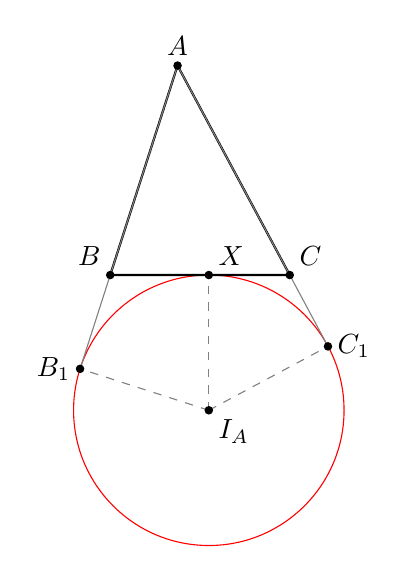
\begin{tikzpicture}[scale=0.95]
  \coordinate (A)  at (-0.3,2.8);
  \coordinate (B)  at (-1.2,0);
  \coordinate (C)  at (1.2,0);
  \coordinate (Ia) at (0.118,-1.808);
  \coordinate (X)  at (0.118,0);
  \coordinate (B1) at (-1.603,-1.254);
  \coordinate (C1) at (1.711,-0.954);

  \draw[red] (Ia) circle (1.808);
  \draw[thick] (A) -- (B) -- (C) -- cycle;
  \draw[gray] (A) -- (B1);
  \draw[gray] (A) -- (C1);
  \draw[gray,dashed] (Ia) -- (X);
  \draw[gray,dashed] (Ia) -- (B1);
  \draw[gray,dashed] (Ia) -- (C1);

  \titik{A,B,C,Ia,X,B1,C1}
  \node[above]       at (A)  {$A$};
  \node[above left]  at (B)  {$B$};
  \node[above right] at (C)  {$C$};
  \node[below right] at (Ia) {$I_A$};
  \node[above right] at (X)  {$X$};
  \node[left]        at (B1) {$B_1$};
  \node[right]       at (C1) {$C_1$};
\end{tikzpicture}
\caption{Panjang garis singgung dari $A$ ke $A$-excircle sama dengan setengah keliling.}
\end{figure}

\begin{proof}
Panjang dua garis singgung dari satu titik ke sebuah lingkaran selalu sama, jadi $AB_1 = AC_1$. Misalkan $X$ titik singgung $A$-excircle dengan $BC$. Dengan alasan yang sama, $BB_1 = BX$ dan $CC_1 = CX$. Maka
\begin{align*}
  AB_1 + AC_1 &= (AB + BB_1) + (AC + CC_1) \\
              &= (AB + BX) + (AC + CX) \\
              &= AB + AC + BC = 2s.
\end{align*}
Karena kedua panjang itu sama dan jumlahnya $2s$, masing masing bernilai $s$.
\end{proof}

Dari sini mengalir sederet akibat yang sering dipakai: $BX = s - c$, $CX = s - b$, dan titik singgung lingkaran dalam pada $BC$ merupakan pencerminan $X$ terhadap titik tengah $BC$.

\subsection{Latihan Soal Homothety}

\begin{enumerate}
  \item Buktikan bahwa titik berat segitiga membagi setiap garis berat dengan rasio $2:1$, lalu jelaskan homoteti mana yang dipakai.

  \item (Garis Euler) Pada segitiga $ABC$, misalkan $O$, $G$, $H$, dan $N_9$ berturut turut titik pusat lingkaran luar, titik berat, titik tinggi, dan pusat lingkaran sembilan titik. Buktikan keempatnya segaris, dan $G$ membagi $OH$ dengan rasio $2:1$.

  \item Buktikan lemma lingkaran sembilan titik: titik tengah ketiga sisi, ketiga kaki garis tinggi, dan titik tengah $AH$, $BH$, $CH$ terletak pada satu lingkaran berjari jari $R/2$.

  \item (OSN 2018) Misalkan $\Gamma_1$ dan $\Gamma_2$ dua lingkaran yang bersinggungan di titik $A$ dengan $\Gamma_2$ di dalam $\Gamma_1$. Misalkan $B$ titik pada $\Gamma_2$ dan garis $AB$ memotong $\Gamma_1$ di titik $C$. Misalkan $D$ titik pada $\Gamma_1$ dan $P$ sebarang titik pada garis $CD$, boleh pada perpanjangan segmen $CD$. Garis $BP$ memotong $\Gamma_2$ di titik $Q$. Tunjukkan bahwa $A$, $D$, $P$, $Q$ terletak pada satu lingkaran.

  \item (OSN 2022) Pada segitiga $ABC$, titik $D$ dan $E$ berada pada sisi $AB$ dan $AC$ sehingga $DE \parallel BC$. Diketahui terdapat titik $P$ di interior segiempat $BDEC$ dengan $\angle BPD = \angle CPE = 90^\circ$. Buktikan bahwa garis $AP$ melalui titik pusat lingkaran luar segitiga $EPD$ dan segitiga $BPC$.

  \item Diberikan segitiga $ABC$ dengan lingkaran luar $\Omega$ dan titik $D$ pada $BC$. Gambar lingkaran yang menyinggung $AD$ di $L$, menyinggung $BC$ di $K$, dan menyinggung $\Omega$ dari dalam. Tunjukkan bahwa titik pusat lingkaran dalam $\triangle ABC$ terletak pada $KL$.

  \item (Philippine 2022) In $\triangle ABC$, let $D$ be the point on side $BC$ such that $AB + BD = DC + CA$. The line $AD$ intersects the circumcircle of $\triangle ABC$ again at point $X \neq A$. Prove that one of the common tangents of the circumcircles of $\triangle BDX$ and $\triangle CDX$ is parallel to $BC$.

  \item (BAMO 2013) Let $H$ be the orthocenter of an acute triangle $ABC$. Consider the circumcenters of triangles $ABH$, $BCH$, and $CAH$. Prove that they are the vertices of a triangle congruent to $ABC$.

  \item (EGMO 2013) Sisi $BC$ dari segitiga $ABC$ diperpanjang melewati $C$ ke titik $D$ sehingga $CD = BC$. Sisi $CA$ diperpanjang melewati $A$ ke titik $E$ sehingga $AE = 2CA$. Buktikan bahwa jika $AD = BE$, maka $ABC$ segitiga siku siku.

  \item (OSN 2018) Misalkan $I$ dan $O$ berturut turut titik pusat lingkaran dalam dan lingkaran luar segitiga $ABC$. Lingkaran singgung luar $\omega_A$ menyinggung sisi $BC$ di $N$ serta menyinggung perpanjangan sisi $AB$ dan $AC$ masing masing di $K$ dan $M$. Jika titik tengah ruas garis $KM$ berada pada lingkaran luar segitiga $ABC$, buktikan bahwa $O$, $I$, dan $N$ segaris.
\end{enumerate}

\newpage
\section{Length Chasing}

\subsection{Kuasa Titik}

\begin{definition*}
Kuasa titik $P$ terhadap lingkaran $\omega$ berpusat $O$ dan berjari jari $r$ adalah
\[
\operatorname{Pow}_\omega(P) = OP^2 - r^2.
\]
Nilainya positif kalau $P$ di luar $\omega$, nol kalau $P$ pada $\omega$, dan negatif kalau $P$ di dalam $\omega$.
\end{definition*}

\begin{theorem*}
Jika sebuah garis melalui $P$ memotong $\omega$ di $X$ dan $Y$, maka
\[
PX \cdot PY = \left| \operatorname{Pow}_\omega(P) \right|.
\]
Khususnya, kalau $P$ di luar $\omega$ dan $PT$ menyinggung $\omega$ di $T$, maka $PT^2 = \operatorname{Pow}_\omega(P)$.
\end{theorem*}

\begin{figure}[H]
\centering
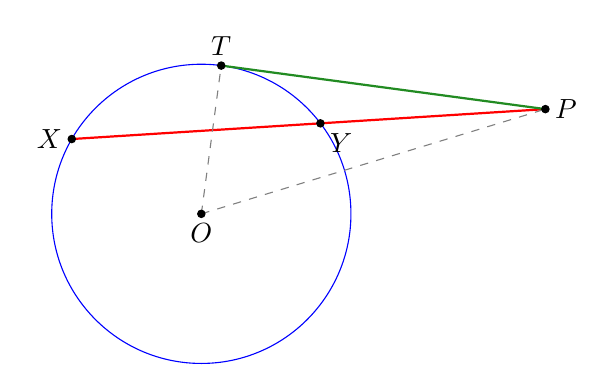
\begin{tikzpicture}[scale=0.95]
  \coordinate (O) at (0,0);
  \coordinate (P) at (4.6,1.4);
  \coordinate (X) at (-1.732,1.000);
  \coordinate (Y) at (1.592,1.210);
  \coordinate (T) at (0.266,1.982);

  \draw[blue] (O) circle (2);
  \draw[red,thick] (P) -- (X);
  \draw[ForestGreen,thick] (P) -- (T);
  \draw[gray,dashed] (O) -- (T);
  \draw[gray,dashed] (O) -- (P);

  \titik{O,P,X,Y,T}
  \node[below]       at (O) {$O$};
  \node[right]       at (P) {$P$};
  \node[left]        at (X) {$X$};
  \node[below right] at (Y) {$Y$};
  \node[above]       at (T) {$T$};
\end{tikzpicture}
\caption{$PX \cdot PY = PT^2 = OP^2 - r^2$.}
\end{figure}

\begin{theorem*}[Kebalikan kuasa titik]
Misalkan $A$, $B$, $X$, $Y$ empat titik berbeda, dan garis $AB$ serta $XY$ berpotongan di $P$. Jika $PA \cdot PB = PX \cdot PY$ dengan $P$ terletak sama sama di dalam atau sama sama di luar kedua ruas garis, maka $A$, $B$, $X$, $Y$ konsiklis.
\end{theorem*}

Teorema kebalikan ini yang paling sering menyelamatkan soal. Kalau kalian sudah punya kesamaan hasil kali panjang tetapi belum punya lingkaran, kesiklisan biasanya tinggal diambil.

\subsubsection{Sumbu Radikal}

Sumbu radikal dua lingkaran $\omega_1$ dan $\omega_2$ yang berpusat di $O_1$ dan $O_2$ adalah tempat kedudukan titik yang kuasanya terhadap kedua lingkaran sama besar. Tempat kedudukan itu berupa garis lurus yang tegak lurus $O_1O_2$. Kalau kedua lingkaran berpotongan di $A$ dan $B$, sumbu radikalnya persis garis $AB$.

\begin{figure}[H]
\centering
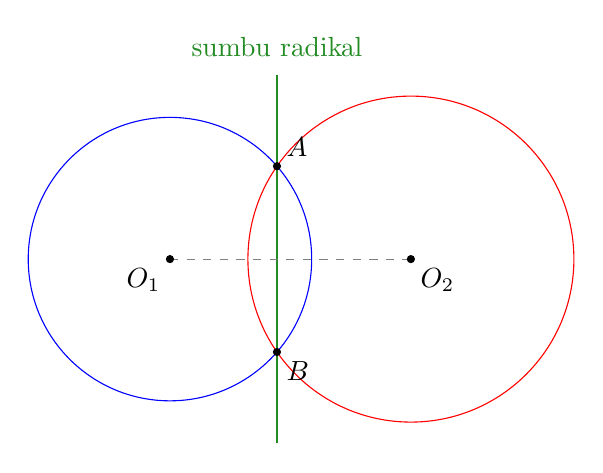
\begin{tikzpicture}[scale=0.9]
  \coordinate (O1) at (0,0);
  \coordinate (O2) at (3.4,0);
  \coordinate (A)  at (1.510,1.311);
  \coordinate (B)  at (1.510,-1.311);

  \draw[blue] (O1) circle (2);
  \draw[red] (O2) circle (2.3);
  \draw[ForestGreen,thick] (1.510,2.6) -- (1.510,-2.6);
  \draw[gray,dashed] (O1) -- (O2);

  \titik{O1,O2,A,B}
  \node[below left]  at (O1) {$O_1$};
  \node[below right] at (O2) {$O_2$};
  \node[above right] at (A)  {$A$};
  \node[below right] at (B)  {$B$};
  \node[ForestGreen] at (1.51,3.0) {sumbu radikal};
\end{tikzpicture}
\caption{Sumbu radikal dua lingkaran yang berpotongan.}
\end{figure}

Untuk tiga lingkaran yang pusatnya tidak segaris, ketiga sumbu radikal berpasangan bertemu di satu titik yang disebut \textbf{titik pusat radikal}. Bentuk pakainya di soal biasanya begini: kalau $A$, $B$ pada $\omega_1$ dan $C$, $D$ pada $\omega_2$, maka $A$, $B$, $C$, $D$ konsiklis jika dan hanya jika perpotongan garis $AB$ dan $CD$ terletak pada sumbu radikal $\omega_1$ dan $\omega_2$.

\subsection{Teorema Ceva}

\begin{theorem*}[Ceva]
Pada $\triangle ABC$, misalkan $D$, $E$, $F$ berturut turut pada sisi $BC$, $CA$, $AB$. Garis $AD$, $BE$, $CF$ konkuren jika dan hanya jika
\[
\frac{BD}{DC} \cdot \frac{CE}{EA} \cdot \frac{AF}{FB} = 1.
\]
\end{theorem*}

\begin{theorem*}[Ceva bentuk trigonometri]
Dengan penamaan yang sama, $AD$, $BE$, $CF$ konkuren jika dan hanya jika
\[
\frac{\sin \angle BAD}{\sin \angle DAC} \cdot \frac{\sin \angle ACF}{\sin \angle FCB} \cdot \frac{\sin \angle CBE}{\sin \angle EBA} = 1.
\]
\end{theorem*}

\begin{figure}[H]
\centering
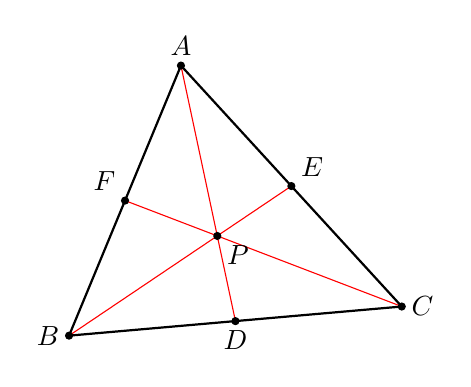
\begin{tikzpicture}[scale=0.9]
  \coordinate (A) at (-0.673,2.511);
  \coordinate (B) at (-2.252,-1.300);
  \coordinate (C) at (2.443,-0.889);
  \coordinate (P) at (-0.160,0.107);
  \coordinate (D) at (0.096,-1.095);
  \coordinate (E) at (0.885,0.811);
  \coordinate (F) at (-1.462,0.606);

  \draw[thick] (A) -- (B) -- (C) -- cycle;
  \draw[red] (A) -- (D);
  \draw[red] (B) -- (E);
  \draw[red] (C) -- (F);

  \titik{A,B,C,D,E,F,P}
  \node[above]       at (A) {$A$};
  \node[left]        at (B) {$B$};
  \node[right]       at (C) {$C$};
  \node[below]       at (D) {$D$};
  \node[above right] at (E) {$E$};
  \node[above left]  at (F) {$F$};
  \node[below right] at (P) {$P$};
\end{tikzpicture}
\caption{Tiga cevian yang konkuren di $P$.}
\end{figure}

\begin{proof}[Bukti bentuk pertama lewat luas]
Tulis $[XYZ]$ untuk luas segitiga $XYZ$, dan misalkan ketiga cevian bertemu di $P$. Segitiga $ABD$ dan $ADC$ punya tinggi sama dari $A$, jadi
\[
\frac{BD}{DC} = \frac{[ABD]}{[ADC]}.
\]
Dengan alasan yang sama $\dfrac{BD}{DC} = \dfrac{[PBD]}{[PDC]}$. Sifat proporsi memberi
\[
\frac{BD}{DC} = \frac{[ABD] - [PBD]}{[ADC] - [PDC]} = \frac{[ABP]}{[ACP]}.
\]
Lakukan hal serupa untuk dua sisi lainnya:
\[
\frac{CE}{EA} = \frac{[BCP]}{[BAP]}, \qquad \frac{AF}{FB} = \frac{[CAP]}{[CBP]}.
\]
Kalikan ketiganya, semua luas saling menghapus, dan hasilnya $1$.
\end{proof}

\subsection{Teorema Menelaus}

\begin{theorem*}[Menelaus]
Diberikan $\triangle ABC$. Sebuah garis memotong garis $BC$, $CA$, $AB$ berturut turut di $D$, $E$, $F$. Maka
\[
\frac{BD}{DC} \cdot \frac{CE}{EA} \cdot \frac{AF}{FB} = 1.
\]
Bentuk ini memakai panjang tanpa tanda. Dengan ruas garis berarah, hasil kalinya bernilai $-1$, dan itulah versi yang membedakan Menelaus dari Ceva.
\end{theorem*}

\begin{figure}[H]
\centering
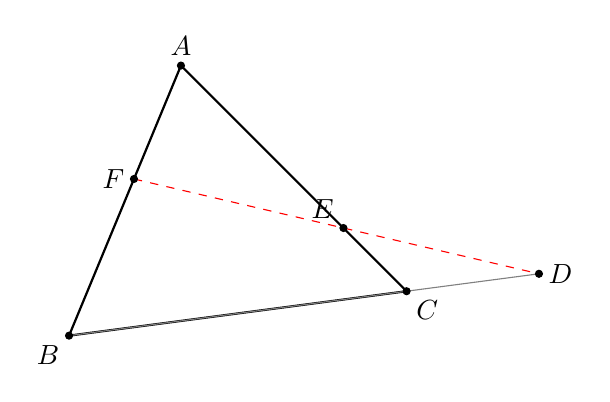
\begin{tikzpicture}[scale=0.9]
  \coordinate (A) at (-0.673,2.511);
  \coordinate (B) at (-2.252,-1.300);
  \coordinate (C) at (2.511,-0.673);
  \coordinate (D) at (4.379,-0.427);
  \coordinate (E) at (1.620,0.219);
  \coordinate (F) at (-1.336,0.911);

  \draw[thick] (A) -- (B) -- (C) -- cycle;
  \draw[gray] (B) -- (D);
  \draw[red,dashed] (F) -- (D);

  \titik{A,B,C,D,E,F}
  \node[above]       at (A) {$A$};
  \node[below left]  at (B) {$B$};
  \node[below right] at (C) {$C$};
  \node[right]       at (D) {$D$};
  \node[above left]  at (E) {$E$};
  \node[left]        at (F) {$F$};
\end{tikzpicture}
\caption{Transversal $DEF$ memotong ketiga garis sisi segitiga.}
\end{figure}

\begin{proof}
Tarik garis tegak lurus dari $A$, $B$, $C$ ke garis transversal $DEF$, dan sebut panjangnya $h_a$, $h_b$, $h_c$. Segitiga siku siku yang terbentuk di $D$ sebangun, jadi $\dfrac{BD}{DC} = \dfrac{h_b}{h_c}$. Dari kesebangunan di $E$ dan di $F$ diperoleh $\dfrac{CE}{EA} = \dfrac{h_c}{h_a}$ dan $\dfrac{AF}{FB} = \dfrac{h_a}{h_b}$. Kalikan ketiganya.
\end{proof}

Cara paling cepat membedakan keduanya saat mengerjakan soal: Ceva mengurus tiga garis yang bertemu di satu titik, Menelaus mengurus tiga titik yang terletak pada satu garis. Kalau soal menyebut kata konkuren, coba Ceva. Kalau soal menyebut kata segaris, coba Menelaus.

\subsection{Latihan Soal Length Chasing}

\begin{enumerate}
  \item (OSK 2011, 2012, 2013, 2018) Diberikan segitiga $ABC$ dan lingkaran $\Gamma$ berdiameter $AB$. Lingkaran $\Gamma$ memotong sisi $AC$ dan $BC$ berturut turut di $D$ dan $E$. Jika $AD = \frac13 AC$, $BE = \frac14 BC$, dan $AB = 30$, tentukan luas segitiga $ABC$.

  \item (OSP 2018) Misalkan $\Gamma_1$ dan $\Gamma_2$ dua lingkaran berbeda dengan jari jari sama, berpusat di $O_1$ dan $O_2$, dan bersinggungan di titik $P$. Garis $\ell$ melalui $O_1$ menyinggung $\Gamma_2$ di titik $A$, serta memotong $\Gamma_1$ di titik $X$ dengan $X$ di antara $A$ dan $O_1$. Misalkan $M$ titik tengah $AX$ dan $Y$ titik potong $PM$ dengan $\Gamma_2$, dengan $Y \neq P$. Buktikan bahwa $XY$ sejajar $O_1O_2$.

  \item (OSN 2019) Diberikan lingkaran berpusat $O$. Titik $A$ di dalam lingkaran namun bukan pada kelilingnya, dan $B$ pencerminan $A$ terhadap $O$. Sebarang titik $P$ terletak pada keliling lingkaran. Garis yang tegak lurus $AP$ dan melalui $P$ memotong lingkaran di $Q$. Buktikan bahwa $AP \times BQ$ konstan selama $P$ bergerak pada lingkaran.

  \item (Teorema Pitot) Diberikan segiempat $ABCD$. Buktikan bahwa jika ada lingkaran yang termuat di dalamnya dan menyinggung keempat sisinya, maka $AB + CD = BC + DA$.

  \item Pada segitiga $ABC$, titik $D$, $E$, $F$ berturut turut terletak pada segmen $BC$, $CA$, $AB$. Misalkan $P$ perpotongan $AD$ dan $EF$. Tunjukkan bahwa
  \[
  \frac{AB}{AF} \cdot CD + \frac{AC}{AE} \cdot BD = \frac{AD}{AP} \cdot BC.
  \]

  \item Diberikan segitiga $ABC$. Titik $D$ dan $E$ pada segmen $AB$ memenuhi $AE = ED = DB$, dan titik $F$ dan $G$ pada segmen $AC$ memenuhi $AF = FG = GC$. Garis $BF$ memotong $CD$ dan $CE$ berturut turut di $K$ dan $L$, sedangkan garis $BG$ memotong $CD$ dan $CE$ berturut turut di $N$ dan $M$. Buktikan bahwa $KM$ sejajar $BC$.

  \item Diberikan trapesium $ABCD$ dengan $AD \parallel BC$ dan $AB$ tidak sejajar $CD$. Garis $AB$ dan $CD$ berpotongan di $Q$, sedangkan $AC$ dan $BD$ berpotongan di $P$. Buktikan bahwa garis $PQ$ melalui titik tengah $BC$ dan titik tengah $AD$.

  \item (OSN 2013) Diberikan segitiga lancip $ABC$ dengan lingkaran luar $\omega$. Garis bagi $\angle BAC$ memotong $\omega$ lagi di titik $M$. Misalkan $P$ titik pada $AM$ dan di dalam segitiga $ABC$. Garis melalui $P$ yang sejajar $AB$ dan garis melalui $P$ yang sejajar $AC$ memotong $BC$ berturut turut di $E$ dan $F$. Garis $ME$ dan $MF$ memotong $\omega$ berturut turut di $K$ dan $L$. Buktikan bahwa $AM$, $BL$, $CK$ konkuren.

  \item (OSP 2020) Diketahui segitiga $ABC$ tidak sama kaki dengan garis tinggi $AA_1$, $BB_1$, $CC_1$. Misalkan $B_A$ dan $C_A$ berturut turut pada $BB_1$ dan $CC_1$ sehingga $A_1B_A \perp BB_1$ dan $A_1C_A \perp CC_1$. Garis $B_AC_A$ dan $BC$ berpotongan di $T_A$. Definisikan $T_B$ dan $T_C$ dengan cara serupa. Buktikan bahwa $T_A$, $T_B$, $T_C$ kolinear.

  \item (OSN 2023) Diberikan segitiga $ABC$ dengan $\angle ACB = 90^\circ$ dan lingkaran luar $\omega$. Garis singgung $\omega$ di $B$ dan di $C$ bertemu di $P$. Misalkan $M$ titik tengah $PB$. Garis $CM$ memotong $\omega$ di $N$, dan garis $PN$ memotong $AB$ di $E$. Titik $D$ pada $CM$ memenuhi $ED \parallel BM$. Buktikan bahwa lingkaran luar $CDE$ menyinggung $\omega$.

  \item (IMO 2008) Misalkan $H$ titik tinggi segitiga lancip $ABC$. Lingkaran $\Gamma_A$ berpusat di titik tengah $BC$ dan melalui $H$ memotong garis $BC$ di titik $A_1$ dan $A_2$. Definisikan $B_1$, $B_2$, $C_1$, $C_2$ dengan cara serupa. Buktikan bahwa keenam titik tersebut konsiklis.

  \item (USAMO 1997) Diberikan segitiga $ABC$. Ambil titik $D$, $E$, $F$ berturut turut pada sumbu sumbu $BC$, $CA$, $AB$. Tunjukkan bahwa garis melalui $A$ tegak lurus $EF$, garis melalui $B$ tegak lurus $FD$, dan garis melalui $C$ tegak lurus $DE$ konkuren.
\end{enumerate}

\section*{Referensi}
\begin{itemize}
  \item Evan Chen, \emph{Euclidean Geometry in Mathematical Olympiads}, MAA Press, 2016.
  \item Yufei Zhao, \emph{Lemmas in Euclidean Geometry}, \url{https://web.mit.edu/yufeiz/www/olympiad/geolemmas.pdf}
  \item Evan Chen, \emph{Directed Angles}, \url{https://web.evanchen.cc/handouts/Directed-Angles/Directed-Angles.pdf}
\end{itemize}

\end{document}
